\section{Structures et matériaux}

%https://fr.wikipedia.org/wiki/Configuration_d%27aile
%https://fr.wikipedia.org/wiki/Profil_(a%C3%A9rodynamique)
%en.wikipedia.org/wiki/Airfoil
%https://fr.wikipedia.org/wiki/Portance_(a%C3%A9rodynamique)
%https://fr.wikipedia.org/wiki/Phare_et_feu_(a%C3%A9ronautique)#:~:text=Ils%20sont%20g%C3%A9n%C3%A9ralement%20situ%C3%A9s%20aux,la%20queue%20de%20l'avion.
%https://en.wikipedia.org/wiki/Drag_(physics)#Aerodynamics

\subsection{La cellule d'un avion}
	\begin{figure}[H]
  		\centering
    		\includegraphics[width=1.0\textwidth]{01-EtudeAeronefs/img/celluleAvionLegendee.pdf}
    		%\scalebox{0.8}{% Source de l'image : https://en.wikipedia.org/wiki/Airframe#/media/File:RV-14_Cutaway_TD_-_small.jpg
% Ajout des flèches pour l'illustration
% Licence CC BY-SA 4.0
\documentclass{standalone}

\usepackage{xcolor}
\usepackage{tikz}


\begin{document}

\usetikzlibrary{calc,fit,backgrounds}
\tikzset{>=latex} % for LaTeX arrow head
\colorlet{mydarkblue}{blue!30!black}
\tikzstyle{arrow}=[<-,very thick,mydarkblue]
\tikzstyle{vector}=[->,line width=2,green!50!black]
\definecolor{fond}{HTML}{fdfdff}
\begin{tikzpicture}[background rectangle/.style={fill=fond!100}, show background rectangle]
\node[inner sep=0pt] (cellule) at (0,0)
    {\includegraphics[width=1.0\textwidth]{celluleAvion.jpg}};
    %{\includegraphics[width=1.0\textwidth]{01-EtudeAeronefs/img/celluleAvion.jpg}};
    
    %\draw[arrow] (0,0) ++ (-.2,.2) --++ (-3,-1.5)
    %node[below left=-2,align=right,scale=1.4] {reférence};
    
    \draw[arrow] (-3,1) ++ (-.2,.2) --++ (-3,-1.5)
    node[below left=-2,align=right,scale=1.4] {moteur};
    
    \draw[arrow] (-4.4,2) ++ (-.2,.2) --++ (-2,-1)
    node[below left=-2,align=right,scale=1.4] {hélice};
    
    \draw[arrow] (-0.8,-1.6) ++ (-.2,.2) --++ (-3,-1.5)
    node[below left=-2,align=right,scale=1.4] {train d'atterissage};
    
    \draw[arrow] (3.8,3.5) ++ (-.2,.2) --++ (-1,1.5)
    node[above left=-2,align=right,scale=1.4] {dérive};
    
    \draw[arrow] (-1,2.2) ++ (-.2,.2) --++ (-1,1.5)
    node[above left=-2,align=right,scale=1.4] {cockpit};
    
    \draw[arrow] (1,2.2) ++ (-.2,.2) --++ (-2,3)
    node[above left=-2,align=right,scale=1.4] {fuselage};
    
    \draw[arrow] (4.3,3.5) ++ (-.2,.2) --++ (3,-1.5)
    node[below right=-2,align=right,scale=1.4] {gouverne de\\[-2pt]direction};
    
    \draw[arrow] (5,1.7) ++ (-.2,.2) --++ (2.25,-1.125)
    node[below right=-2,align=right,scale=1.4] {gouverne de\\[-2pt]profondeur};
    
    \draw[arrow] (1,0.2) ++ (-.2,.2) --++ (3,0)
    node[below right=-2,align=right,scale=1.4] {volet};
    
    \draw[arrow] (3.5,-1.2) ++ (-.2,.2) --++ (3,0)
    node[below right=-2,align=right,scale=1.4] {aileron};
    
    \draw[arrow] (2.2,-1.5) ++ (-.2,.2) --++ (-6,-3)
    node[below left=-2,align=right,scale=1.4] {aile};
    
    %\draw (-8,-8) grid (8,8);

\end{tikzpicture}

\end{document}}
  		\legende{Principaux éléments d'une cellule d'avion}{img:celluleAvionLegendee}
	\end{figure}	
	
\subsubsection{L'aile}
 	Toutes les ailes \anglais{wing} des avions sont globalement conçues selon les mêmes principes.
 	
 	L'aile est construite autour d'un longeron, poutre maitresse qui permet de transférer la charge portée par l'aile au fuselage. Les nervures \anglais{rib} donnent à l'aile son profil. On fixe sur ces longerons la peau \anglais{skin}, qui constitue la partie visible de l'aile. Des raidisseurs permettent de donner une plus grande rigidité à l'aile.
 	\begin{figure}[H]
  		\centering
    		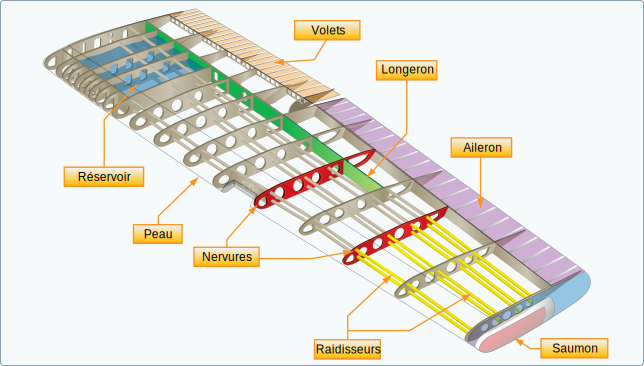
\includegraphics[width=0.75\textwidth]{01-EtudeAeronefs/img/schemaAile.pdf}
  		\legende{Les constituants d'une aile d'avion}{img:schemaAile}
	\end{figure}	
	
	En bout d'aile, le saumon \anglais{wing tip} accueille généralement des feux de navigation.
	
	Sur le bord de fuite et sur la partie extérieure de l'aile sont disposés les ailerons, qui permettent le contrôle en roulis de l'avion. On dispose les volets \anglais{flap} sur le bord de fuite de l'aile du côté du fuselage.
		
\subsection{Différentes conceptions d'ailes}
Au fil de l'histoire de l'aéronautique, de nombreuses formules de dispositions d'ailes ont été proposées pour répondre aux différents besoins. Dans cette partie, nous présenterons les formules les plus emblématiques.

	\subsubsection{Nombre d'ailes}
	Au début de l'histoire de l'aviation, les concepteurs ont massivement recours à des conceptions multiplans. L'intérêt de cette formule est d'augmenter la surface portante en limitant l'envergure de l'aéronef. En effet, les techniques de l'époque ne permettaient pas de concevoir des structures d'ailes de grande longueur. Les formules multiplans permettent par ailleurs d'augmenter la rigidité en reliant les plans entre eux grâce à des filins.
	
\begin{table}[H]
  \centering
  \begin{tabular}{c c c}
    \begin{minipage}{.3\textwidth}
      \begin{figure}[H]
  		\centering
  		\includegraphics[width=1.0\textwidth]{01-EtudeAeronefs/img/ailes/Monoplane_mid.pdf}
  				\legende{Monoplan}{wing:Monoplane-mid}	
		\end{figure}
    \end{minipage}
    &
    \begin{minipage}{.3\textwidth}
      \begin{figure}[H]
  		\centering
  		\includegraphics[width=1.0\textwidth]{01-EtudeAeronefs/img/ailes/Biplane_wire.pdf}
  				\legende{Biplan}{wing:Biplane-wire}		
		\end{figure}
    \end{minipage}
    & 
    \begin{minipage}{.3\textwidth}
      \begin{figure}[H]
  		\centering
  		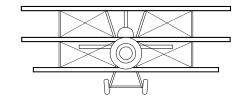
\includegraphics[width=1.0\textwidth]{01-EtudeAeronefs/img/ailes/Triplane.pdf}
  				\legende{Triplan}{wing:Triplane}			
		\end{figure}
    \end{minipage} \\
	\begin{minipage}{.3\textwidth}
      \begin{figure}[H]
  		\centering
  		\includegraphics[width=1.0\textwidth]{01-EtudeAeronefs/img/DR400.jpg}
  			\legende{Monoplan moderne DR400}{img:DR400}	
		\end{figure}
    \end{minipage}
    &
    \begin{minipage}{.3\textwidth}
      \begin{figure}[H]
  		\centering
  		\includegraphics[width=1.0\textwidth]{05-Histoire/img/wrightFlyer.jpg}
  			\legende{Biplan Wright Flyer}{img:wrightFlyer}
		\end{figure}
    \end{minipage}
    & 
    \begin{minipage}{.3\textwidth}
      \begin{figure}[H]
  		\centering
  		\includegraphics[width=1.0\textwidth]{05-Histoire/img/sopwithTriplane.jpg}
  			\legende{Triplan Sopwith Triplane}{img:sopwithTriplane}			
		\end{figure}
    \end{minipage}
  \end{tabular}
  %\caption{}
\end{table}

\begin{table}[H]
  \centering
  \begin{tabular}{c c}
    \begin{minipage}{.3\textwidth}
      \begin{figure}[H]
  		\centering
  		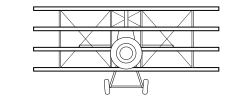
\includegraphics[width=1.0\textwidth]{01-EtudeAeronefs/img/ailes/Quadruplane.pdf}
  				\legende{Quadriplan}{wing:Quadruplane}		
		\end{figure}
    \end{minipage}
    &
    \begin{minipage}{.3\textwidth}
      \begin{figure}[H]
  		\centering
  		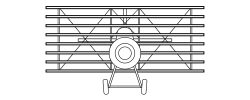
\includegraphics[width=1.0\textwidth]{01-EtudeAeronefs/img/ailes/Multiplane.pdf}
  				\legende{Multiplan}{wing:Multiplane}			
		\end{figure}
    \end{minipage} \\
	\begin{minipage}{.3\textwidth}
      \begin{figure}[H]
  		\centering
  		\includegraphics[width=1.0\textwidth]{05-Histoire/img/bessonH5.jpg}
  		\legende{Quadriplan Besson H5}{img:bessonH5}	
		\end{figure}
    \end{minipage}
    &
    \begin{minipage}{.3\textwidth}
      \begin{figure}[H]
  		\centering
  		\includegraphics[width=1.0\textwidth]{01-EtudeAeronefs/img/horatioPhillipsMultiplane.png}
  		\legende{Appareil doté de 20 plans (1904)}{img:horatioPhillipsMultiplane}
		\end{figure}
    \end{minipage}
  \end{tabular}
  %\caption{}
\end{table}

On constate que certains concepteurs d'avion sont arrivés sur des formules extrêmes avec un nombre de plan très élevé.

Ces formules multiplans ont finalement été abandonnées car les interactions aérodynamiques entre ailes superposées sont nuisibles : le doublement de la surface de le doublement du nombre d'aile ne multiplie pas par 2 la portance !

 
 	\subsubsection{Dièdre de l'aile}
 	Le dièdre est l'angle formé par le plan de chaque aile et le plan horizontal. Le dièdre à un impact sur la stabilité, notamment en roulis.
 \begin{table}[H]
  \centering
  \begin{tabular}{c c c}
    \begin{minipage}{.3\textwidth}
      \begin{figure}[H]
  		\centering
  		\includegraphics[width=1.0\textwidth]{01-EtudeAeronefs/img/ailes/Monoplane_dihedral.pdf}
  		\legende{Dièdre positif}{wing:Monoplane-dihedral}		
		\end{figure}
    \end{minipage}
    &
    \begin{minipage}{.3\textwidth}
      \begin{figure}[H]
  		\centering
  		\includegraphics[width=1.0\textwidth]{01-EtudeAeronefs/img/ailes/Monoplane_mid.pdf}
  		\legende{Dièdre nul}{wing:Monoplane-mid}			
		\end{figure}
    \end{minipage} 
    &
    \begin{minipage}{.3\textwidth}
      \begin{figure}[H]
  		\centering
  		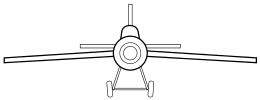
\includegraphics[width=1.0\textwidth]{01-EtudeAeronefs/img/ailes/Monoplane_anhedral.pdf}
  		\legende{Dièdre négatif}{wing:Monoplane-anhedral}		
		\end{figure}
    \end{minipage}\\
	\begin{minipage}{.3\textwidth}
      \begin{figure}[H]
  		\centering
  		\includegraphics[width=1.0\textwidth]{01-EtudeAeronefs/img/B737.jpg}
  		\legende{Boeing 737}{img:B737}		
		\end{figure}
    \end{minipage}
    &
    \begin{minipage}{.3\textwidth}
      \begin{figure}[H]
  		\centering
  		\includegraphics[width=1.0\textwidth]{01-EtudeAeronefs/img/cap232.jpg}
  		\legende{Cap 232}{img:cap232}
		\end{figure}
    \end{minipage}
    &
    \begin{minipage}{.3\textwidth}
      \begin{figure}[H]
  		\centering
  		\includegraphics[width=1.0\textwidth]{01-EtudeAeronefs/img/An124.jpg}
  		\legende{Antono 124}{img:An124}		
		\end{figure}
    \end{minipage}
  \end{tabular}
  %\caption{}
\end{table}
	
	\subsubsection{Forme d'ailes}
	Au delà du dièdre ou du nombre de plans, les ingénieurs aéronautiques ont conçu de nombreuses formes d'ailes pour répondre aux besoins propres de chaque type de machine : une aile ne pourra pas avoir la même forme si l'objectif est d'emmener 4 passagers à quelques centaines de kilomètres par heure, 200 passagers à 800 km, 100 passagers à Mach 2 ou de l'armement depuis un avion embarqué sur un porte-avion.
	
\begin{table}[H]
  \centering
  \begin{tabular}{c c c}
    \begin{minipage}{.3\textwidth}
      \begin{figure}[H]
  		\centering
  		\includegraphics[width=1.0\textwidth]{01-EtudeAeronefs/img/ailes/Wing_constant.pdf}
  			\legende{Aile rectangulaire}{wing:Wing-constant}		
		\end{figure}
    \end{minipage}
    &
    \begin{minipage}{.3\textwidth}
      \begin{figure}[H]
  		\centering
  		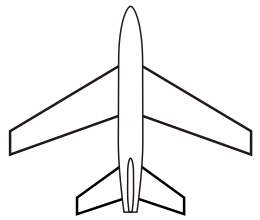
\includegraphics[width=1.0\textwidth]{01-EtudeAeronefs/img/ailes/Wing_swept.pdf}
  			\legende{Aile en flèche}{wing:Wing-swept}				
		\end{figure}
    \end{minipage} 
    &
    \begin{minipage}{.3\textwidth}
      \begin{figure}[H]
  		\centering
  		\includegraphics[width=1.0\textwidth]{01-EtudeAeronefs/img/ailes/Wing_elliptical.pdf}
  			\legende{Aile elliptique}{wing:Wing-elliptical}		
		\end{figure}
    \end{minipage}\\
	\begin{minipage}{.3\textwidth}
      \begin{figure}[H]
  		\centering
  		\includegraphics[width=1.0\textwidth]{01-EtudeAeronefs/img/pilatusPC6.jpg}
  			\legende{Pilatus PC6}{img:pilatusPC6}		
		\end{figure}
    \end{minipage}
    &
    \begin{minipage}{.3\textwidth}
      \begin{figure}[H]
  		\centering
  		\includegraphics[width=1.0\textwidth]{01-EtudeAeronefs/img/A380.jpg}
  		\legende{Avion de ligne}{img:A380}
		\end{figure}
    \end{minipage}
    &
    \begin{minipage}{.3\textwidth}
      \begin{figure}[H]
  		\centering
  		\includegraphics[width=1.0\textwidth]{05-Histoire/img/spitfire.jpg}
  		\legende{Un Spitfire}{img:spitfire}
		\end{figure}
    \end{minipage}
  \end{tabular}
  %\caption{}
\end{table}
	
\begin{table}[H]
  \centering
  \begin{tabular}{c c c}
    \begin{minipage}{.3\textwidth}
      \begin{figure}[H]
  		\centering
  		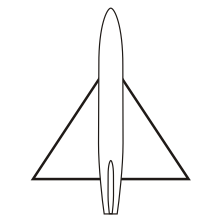
\includegraphics[width=1.0\textwidth]{01-EtudeAeronefs/img/ailes/Wing_tailless_delta.pdf}
  		\legende{Aile delta}{wing:Wing-tailless-delta}	
		\end{figure}
    \end{minipage}
    &
    \begin{minipage}{.3\textwidth}
      \begin{figure}[H]
  		\centering
  		\includegraphics[width=1.0\textwidth]{01-EtudeAeronefs/img/ailes/Wing_ogival_delta.pdf}
  		\legende{Aile gothique}{wing:Wing-ogival-delta}	
		\end{figure}
    \end{minipage}
    & 
    \begin{minipage}{.3\textwidth}
      \begin{figure}[H]
  		\centering
  		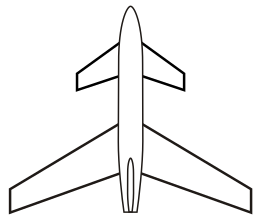
\includegraphics[width=1.0\textwidth]{01-EtudeAeronefs/img/ailes/Wing_canard.pdf}
  		\legende{Configuration canard}{wing:Wing-canard}		
		\end{figure}
    \end{minipage} \\
	\begin{minipage}{.3\textwidth}
      \begin{figure}[H]
  		\centering
  		\includegraphics[width=1.0\textwidth]{01-EtudeAeronefs/img/mirage2000.jpg}
  		\legende{Aile delta : chasseur}{img:mirage2000}	
		\end{figure}
    \end{minipage}
    &
    \begin{minipage}{.3\textwidth}
      \begin{figure}[H]
  		\centering
  		\includegraphics[width=1.0\textwidth]{01-EtudeAeronefs/img/concorde.jpg}
  		\legende{Aile gothique : Concorde}{img:concorde}	
		\end{figure}
    \end{minipage}
    & 
    \begin{minipage}{.3\textwidth}
      \begin{figure}[H]
  		\centering
  		\includegraphics[width=1.0\textwidth]{01-EtudeAeronefs/img/rutanLongEz.jpg}
  		\legende{Canard : Long EZ}{img:rutanLongEz}		
		\end{figure}
    \end{minipage}
  \end{tabular}
  %\caption{}
\end{table}
	
	\subsection{Train d'atterrissage}
	\subsubsection{Train classique vs. train tricycle}
	Les premiers avions étaient équipés de trains dits classiques \anglais{taildragger}, avec un train principal généralement équipé de 2 roues à l'avant de l'avion, et une roulette ou un simple patin sous la dérive. Cette configuration est relativement simple et légère, mais présente plusieurs inconvénients :
	\begin{itemize}
		\item l'hélice n'est pas protégée : un freinage trop brutal ou une erreur de contrôle du tangage en phase de décollage peut provoquer le contact de l'hélice avec le sol, voire le basculement de l'avion sur le nez (mise en pylône) ou même sur le dos,
		\item réduit la visibilité vers l'avant au roulage. En effet, au roulage, l'assiette de l'avion est positive, ce qui fait que le nez peut masquer une grande partie de ce qui est devant l'avion. Sur certains avions, cela impose au pilote de rouler en faisant des virages, de façon à pouvoir observer l'environnement devant lui\footnote{\href{https://bea.aero/les-enquetes/evenements-notifies/detail/accident-du-beech-c18s-immatricule-hb-gac-et-du-robin-dr400-immatricule-f-gphl-survenu-le-21-05-2022-a-beziers-34/}{Rapport d'accident illustrant ce risque : https://bea.aero/les-enquetes/evenements-notifies/detail/accident-du-beech-c18s-immatricule-hb-gac-et-du-robin-dr400-immatricule-f-gphl-survenu-le-21-05-2022-a-beziers-34/}},
		\item une relative difficulté de contrôle au sol, l'avion ayant tendance à "échapper", notamment lorsque le vent est latéral.
	\end{itemize}
	
	Un autre type de train, dit tricycle, est donc apparu et devient un standard à partir de la fin des années 1950. La roulette est cette fois-ci déplacée à l'avant de l'appareil. Ce type de train corrige les principaux inconvénients du train classique, au prix cependant d'une légère pénalité sur la vitesse pour les avions à train fixe (la roulette de nez est plus imposante qu'une roulette de queue, et produit donc plus de traînée).
	
	\begin{table}[H]
  \centering
  \begin{tabular}{c c}
    \begin{minipage}{.45\textwidth}
      \begin{figure}[H]
  		\centering
  		\includegraphics[width=1.0\textwidth]{01-EtudeAeronefs/img/D140.jpg}
  		\legende{Train classique (D140)}{img:D140}		
		\end{figure}
    \end{minipage}
    &
    \begin{minipage}{.45\textwidth}
      \begin{figure}[H]
  		\centering
  		\includegraphics[width=1.0\textwidth]{01-EtudeAeronefs/img/DR400.jpg}
  		\legende{Train tricycle (DR400)}{img:DR400}			
		\end{figure}
    \end{minipage} 
  \end{tabular}
  %\caption{}
\end{table}

	\subsubsection{Train rentrant}